\subsection{SLDS outperforms AR-HMM in model comparison tests}
\label{sec:slds:3.2.4}

To quantify the difference in AR-HMM and SLDS model performance, we used cross validation to compare each model's ability to accurately identify ground truth states corresponding to sitting, walking, and rearing behaviors (see Section \ref{sec:slds:3.2.5} for more information on how ground truth labels were obtained). Overall, the SLDS correctly identified the ground truth behavior on more frames for each test set (Fig. \ref{fig:slds:4}a; average fraction correct $0.44$ vs. $0.71$, $P$-value = $0.0002$) with lower error (Fig. \ref{fig:slds:4}b; $RMSE$ 1.16 vs. 0.83, $P$-value = $0.0028$). We also examined the models' F1 scores, which capture both model precision (ability to identify \textit{only} the frames belonging to a given state) and recall (ability to identify \textit{all} the frames belonging to a given state), separately for each behavior (Fig. \ref{fig:slds:4}c). In particular, the SLDS substantially outperformed the AR-HMM in its ability to classify stationary (sitting-like) behaviors (0.55 vs. 0.83, $P$-value = $0.00002$). This points to the effectiveness of the denoising process inherent to the SLDS, as with reduced jitter in the joint positions, fewer stationary frames will be mis-identified as motion. It also at least partly explains the SLDS model's overall higher performance, as the stationary state is much more common in the data than rearing or walking. In contrast, the SLDS suffers from worse performance in classifying non-stationary behaviors (walking: 0.40 vs. 0.14, $P$-value = $0.0026$; rearing: 0.17 vs. 0.04, $P$-value = $0.0025$). This may suggest that the effect of the noise term is too strong in the SLDS model or that it is necessary to include additional motion-related features in the model (see further discussion in \ref{sec:slds:discussion}). 

\begin{figure}[t!]
  \begin{center}
    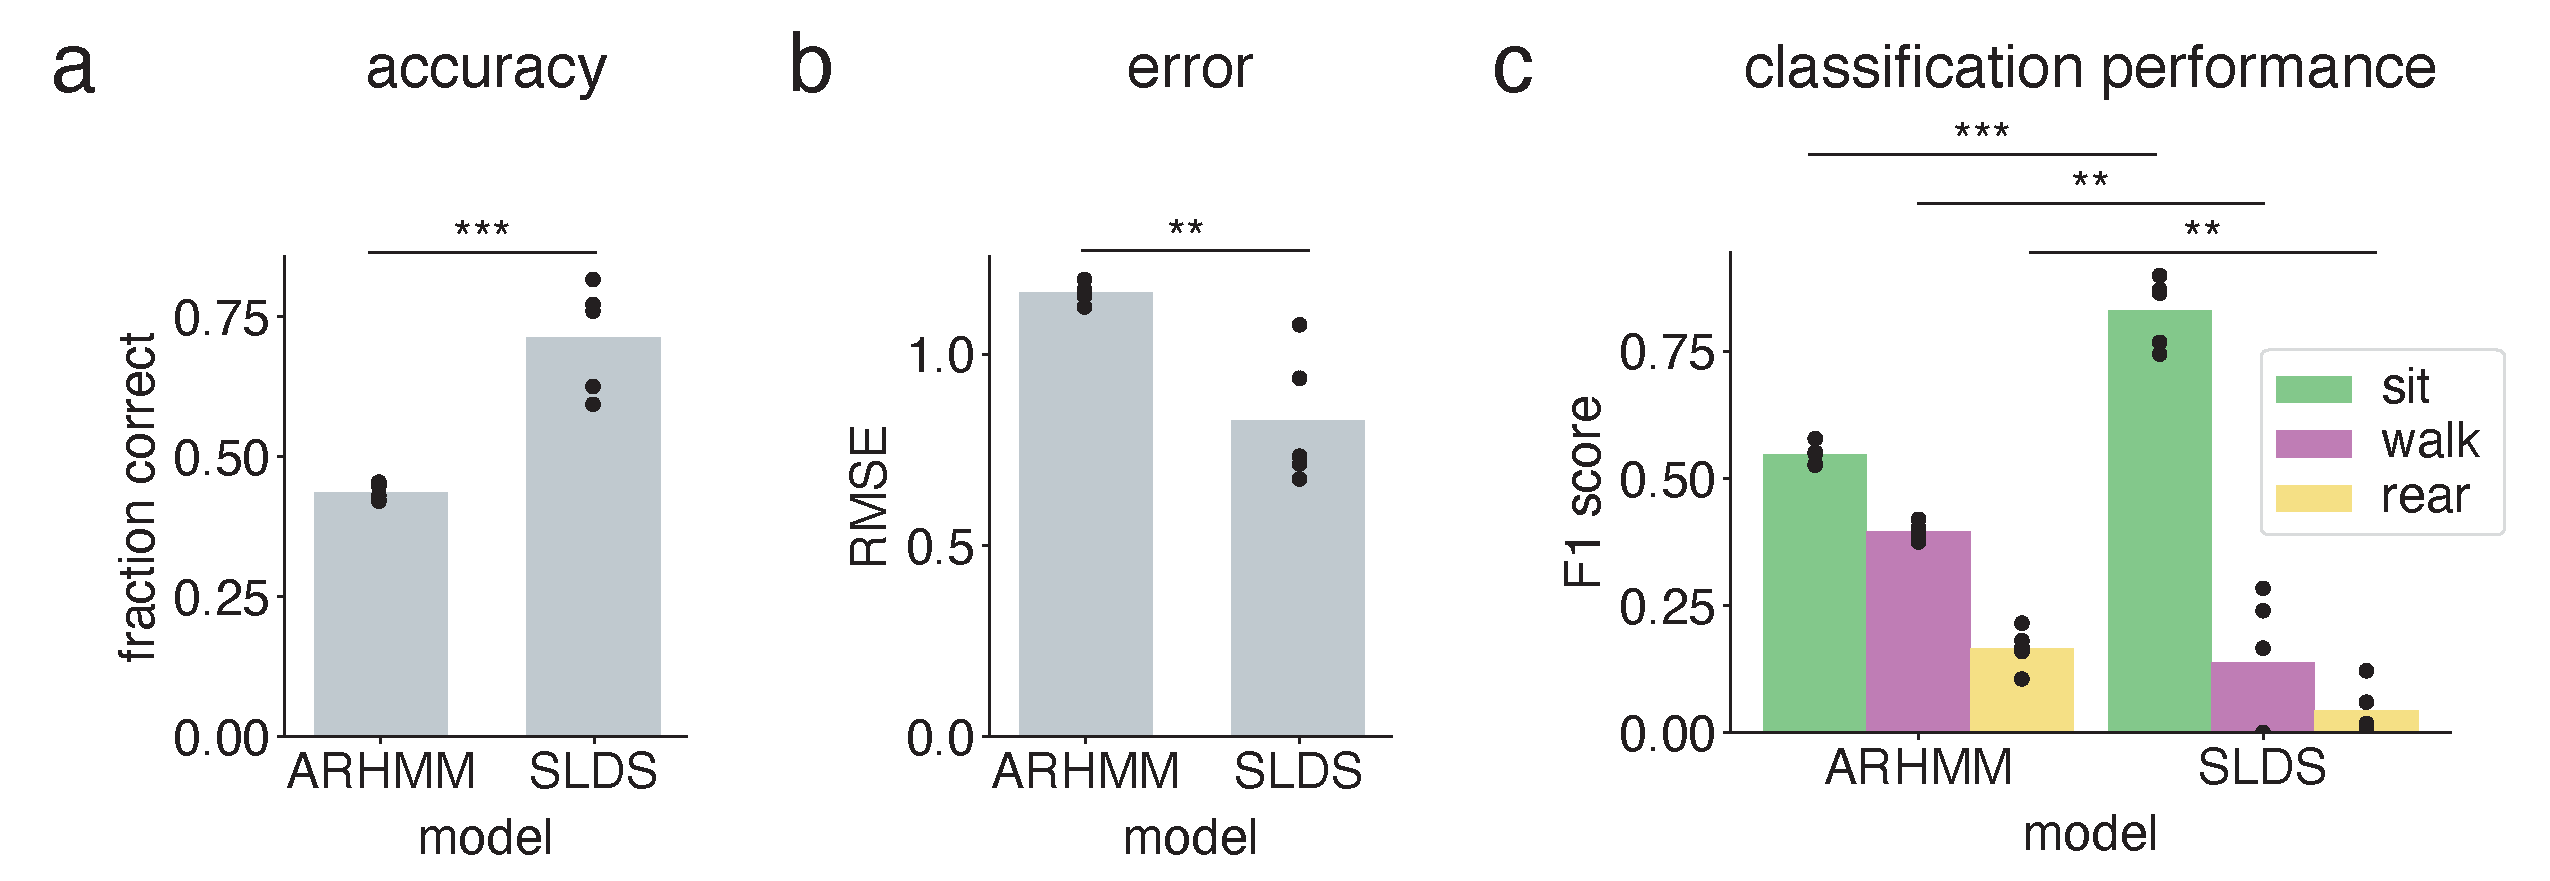
\includegraphics[width=0.90\linewidth]{ch3-slds/slds-figures/Fig4.pdf}
    \caption[Comparison of AR-HMM and SLDS models on multiple metrics]{\textbf{Comparison of AR-HMM and SLDS models on multiple metrics.} (a) Fraction of frames that the AR-HMM and SLDS models correctly labeled as ground truth behaviors (average fraction correct $0.44$ vs. $0.71$, $P$-value = $0.0002$). (b) The root mean square error (RMSE) according to ground truth labels ($RMSE$ 1.16 vs. 0.83, $P$-value = $0.0028$). (c) F1 scores reflecting the model's precision and recall in its ability to classify each ground truth behavior (sitting: 0.55 vs. 0.83, $P$-value = $0.00002$, walking: 0.40 vs. 0.14, $P$-value = $0.0026$; rearing: 0.17 vs. 0.04, $P$-value = $0.0025$). }
    \label{fig:slds:4}
  \end{center}
  \vspace{-0.5cm}
\end{figure}